%% -*- coding: utf-8 -*-
\documentclass[12pt,a4paper]{scrartcl} 
\usepackage[utf8]{inputenc}
\usepackage[english,russian]{babel}
\usepackage{indentfirst}
\usepackage{misccorr}
\usepackage{graphicx}
\usepackage{amsmath}
\usepackage{float}
\usepackage{ dsfont }

\usepackage{xcolor}
\usepackage{hyperref}
\hypersetup{colorlinks,
  pdftitle={The title of your document},
  pdfauthor={Your name},
  allcolors=[RGB]{000 000 000}}

\begin{document}
\begin{titlepage}
  \begin{center}

    Санкт-Петербургский политехнический университет Петра Великого

    \vspace{0.25cm}
    
    Институт прикладной математики и механики
    
    Кафедра «Прикладная математика»
    \vfill

	\vspace{0.25cm}
	    Отчёт\\
	по курсовой работе\\
	по дисциплине\\
	«Вычислительные комплексы»

  \bigskip

\end{center}
\vfill

\newlength{\ML}
\settowidth{\ML}{«\underline{\hspace{0.7cm}}» \underline{\hspace{2cm}}}
\hfill\begin{minipage}{0.4\textwidth}
  Выполнил студент\\ В.\,А.~Рыженко\\
\end{minipage}%
\bigskip

\hfill\begin{minipage}{0.4\textwidth}
  Проверил:\\
к.ф.-м.н., доцент\\
Баженов Александр Николаевич\\
\end{minipage}%
\vfill

\begin{center}
  Санкт-Петербург, 2020 г.
\end{center}
\end{titlepage}

\tableofcontents
%\listoffigures
\newpage


\section{Постановка задачи}

Дана следующая ИСЛАУ:

\begin{equation}
\centering
\begin{pmatrix}
[4; 6] & [-9; 0]& [0; 12]& [2; 3]& [5; 9] &[-23;-9]& [15; 23] &\\
[0; 1] & [6; 10] & [-1; 1]& [-1; 3]& [-5; 1]& [1; 15]& [-3;-1] &\\
[0; 3]& [-20;-9]& [12; 77]& [-6; 30]& [0; 3] &[-18; 1]& [0; 1] &\\
[-4; 1] & [-1; 1] &[-3; 1] &[3; 5] &[5; 9] &[1; 2] &[1; 4]\\
[0; 3] &[0; 6] &[0; 20] &[-1; 5] &[8; 14] &[-6; 1] &[10; 17]\\
[-7;-2] &[1; 2] &[7; 14] &[-3; 1] &[0; 2] &[3; 5] &[-2; 1]\\
[-1; 5] &[-3; 2] &[0; 8] &[1; 11] &[-5; 10] &[2; 7] &[6; 82]
\end{pmatrix} x = 
\begin{pmatrix}
[-10; 95]\\
[35; 14]\\
[-6; 2]\\
[30; 7]\\
[4; 95]\\
[-6; 46]\\
[-2; 65]
\end{pmatrix}
\end{equation}

Если параметризовать матрицу ИСЛАУ $\bold{A}$ следующим образом:

\begin{itemize}
\item   $\bold{a}_{77} = [\gamma, 82]$
\item $\gamma \geq 82$ 
\end{itemize}

То для полученной параметризованной ИСЛАУ решении субдифференциальным методом Ньютона известно. В области значений релаксационного параметра $\tau$ примерно 0.95 имеется резкое увеличение количества необходимых итераций.
Необходимо провести более подробное исследование в окрестности $\gamma$ = 8.

\section {Теория}

\subsection {Субдифференциальный метод Ньютона}

Данный метод используется для решения формальных решений ИСЛАУ вида $\bold{C}x = \bold{d}$, используется техника погружения:

\begin{equation}
sti(x) : (x_1, ..., x_n) \rightarrow (-\underline{x_1}, ... -\underline{x_n}, \underline{x_1}, ..., \underline{x_n})
\end{equation}
и вместо исходной системы решается индуцированное уравнение $\mathcal{G}(x) = 0$. Для начала работы строится некоторое начальное приближение $x^{(0)} \in \mathds{R}^{2n}, k=1,2,...$, уже найдено, то вычисляем какой-нибудь субградиент $D^{(k-1)}$ отбражения $\mathcal{G}$ в точке $x^{(k-1)}$ и полагаем 
\begin{equation}
x^{(k)} \leftarrow x^{(k-1)} - \tau(D^{(k-1)})^{-1}\mathcal{G}(x^{(k-1)})
\end{equation}
где $\tau \in [0, 1]$ некоторая константа, именуемая релаксационным параметром

\section {Реализация}

Лабораторная работа выполнена с помощью пакета прикладных програм Matlab.

\section{Результаты}

Для работы алгоритма было выбрано максимальное количество итераций равное 1000, в действительности при параметрах достигших максимального количества итераций алгоритм расходится и выбранное число является не столь существенным.

Далее рассматриваются графики зависимости количества итераций от парметров $\gamma$ и $\tau$

Рассмотрим первое приближение искомой окрестности

\begin{figure}[H]
    \centering
    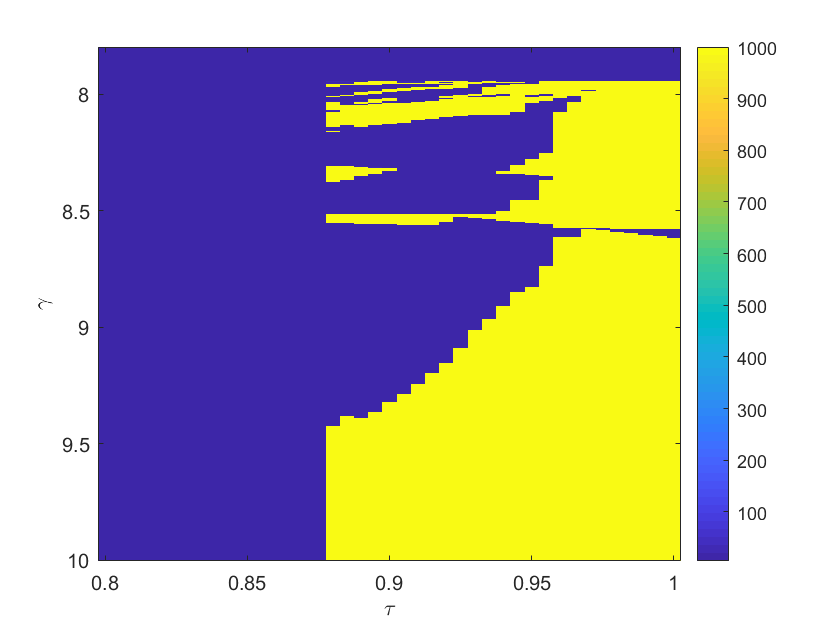
\includegraphics[width=14cm, height=10cm]{fig/1.png}
\end{figure}

Заметна прямоугольная область, вне границ которой алгоритм точно сходится($\tau \lesssim 0.88 \vee  \gamma \lesssim 7.94$), либо точно рассходится($\gamma \gtrsim 9.4 \wedge \tau \gtrsim 0.88$). Рассмотрим эту область.

\begin{figure}[H]
    \centering
    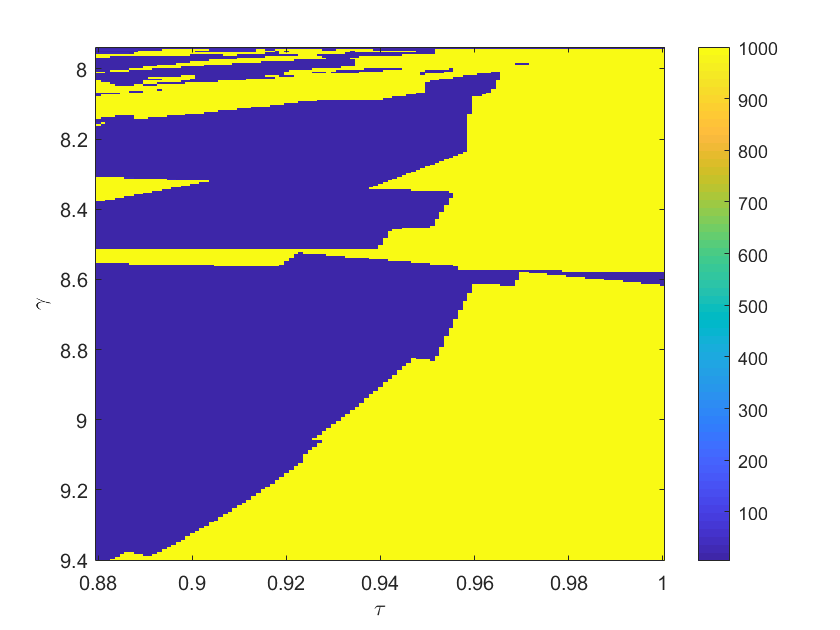
\includegraphics[width=14cm, height=10cm]{fig/2.png}
\end{figure}

Рассмотрим также график где все точки, в которых алгоритм расходится, занулены

\begin{figure}[H]
    \centering
    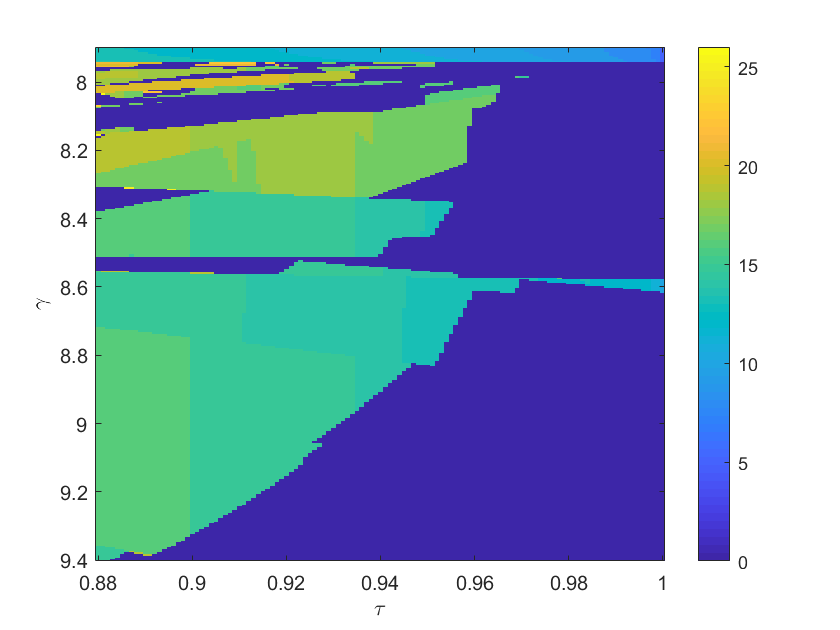
\includegraphics[width=14cm, height=10cm]{fig/3.png}
\end{figure}

Из представленных графиков можно заметить довольно большую область сходимости в окрестности $\gamma = 8.6$, но установить зависмость сходимости затруднительно. Также в этой области алгоритм имеет достаточно хорошую сходимость (до 25 итераций для достижения нормы вектора невязки равной $10^{-7}$).

\section{Приложения}
Репозиторий на GitHub с релизацией: \href{https://github.com/WiillyWonka/Intervals}{github.com}.
\end{document}
